\section{Definition}
\textbf{MapReduce} is a \textbf{popular programming model} designed to \textbf{easily process and generate large datasets on clusters of commodity machines}. Through this paradigm, a computation can be expressed in terms of a \textbf{map and reduce functions} while \textbf{the underlying system deals with communication, parallelization and error handling}, making it easy to use even for programmers who have no experience with distributed systems.

\textbf{Google} created this paradigm in \textbf{2003} in order to reduce development time and cost on their projects; after an analysis of the problem, Google's engineers noticed how \textbf{the majority of the computations in their products could be expressed through the map and reduce abstractions} that are typically present in \textbf{functional languages}. The MapReduce paradigm has been \textbf{used in a variety of Google's project}, including the indexing system used by the Google search engine \cite{google_mapreduce}.

\textbf{\href{https://hadoop.apache.org/}{Apache Hadoop}}, inspired by Google's work, integrates the MapReduce paradigm in its free-licensed framework, making it \textbf{one of the most used options} when it comes to applying distributed computations following this paradigm.

\subsection{The programming model}
In order to execute a MapReduce computation, it is required, as \textbf{input}, \textbf{a set of key/value pairs}. Said values are \textbf{modified through the Map and Reduce functions} and, ultimately, produce as \textbf{output another set of key/value pairs}. 

The Map and Reduce functions are \textbf{written by the user} but in the background, through the framework, behave in the following way:
\begin{itemize}
    \item \textbf{Map}: \textit{(k1, v1) $\Longrightarrow$ list(k2, v2)}\\
    The map function takes a single pair as input and produces a set of intermediate key/value pairs. The framework automatically merges the intermediate sets, grouping them using the keys. Said values are then passed as input to the Reduce function.
    \item \textbf{Reduce}: \textit{(k2, list(v2)) $\Longrightarrow$ list(v2)}\\
    The Reduce function uses the input provided by the automatic merge performed by the framework; every Reduce execution takes a pair of composed of the intermediate key and a collection of values associated to that key. Said pairs are provided using an iterator in order to work with collections that are too large to fit in memory. The values associated to the key are merged to form a possibly smaller set of values, resulting typically in one or zero output values produced as result (even though the function produces a list of values).
\end{itemize}
A programmer that implements a computation following this paradigm does not need to provide anything else but, \textbf{behind the scenes}, the framework performs additional operations such as the \textbf{Splitting} (that divides the input in smaller parts to be executed on the multiple workers) and the \textbf{Shuffling} (that merges the output of the individual Map functions).

Even though the functioning of this paradigm is conceptually easy, the next section analyzes its execution flow with a concrete example.

\subsection{Execution flow}
TODO

\begin{figure}[H]
    \centering
    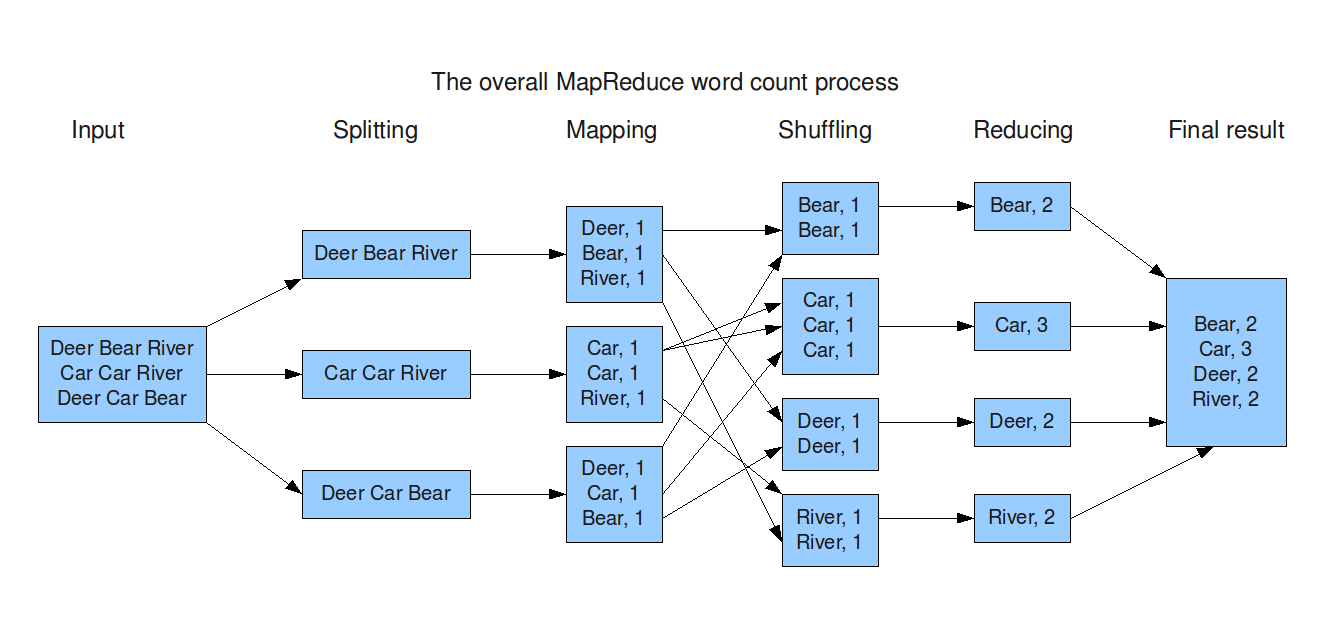
\includegraphics[width=\linewidth]{document/chapters/chapter_4/images/mapreduce_example.png}
    \caption{Example of word count expressed through the MapReduce paradigm \cite{mapreduce_example_site}}
    \label{fig:mapreduce_example}
\end{figure}

\begin{figure}[H]
    \centering
    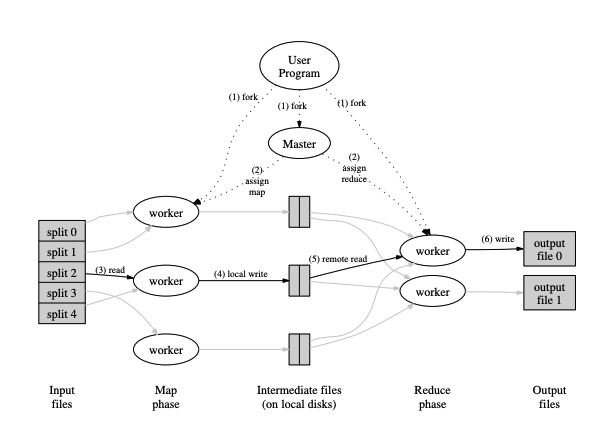
\includegraphics[width=\linewidth]{document/chapters/chapter_4/images/mapreduce_execution_flow.png}
    \caption{MapReduce execution flow \cite{google_mapreduce}}
    \label{fig:mapreduce_execution_flow}
\end{figure}

\subsection{Underlying mechanisms}
TODO

\subsubsection{Data structures}
TODO

\subsubsection{Task granularity}
TODO
% including locality

\subsubsection{Fault tolerance}
TODO
